%
% Modified by Megan Patnott
% Last Change: Jan 18, 2013
%
%%%%%%%%%%%%%%%%%%%%%%%%%%%%%%%%%%%%%%%%%%%%%%%%%%%%%%%%%%%%%%%%%%%%%%%%
%
% Modified by Sameer Vijay
% Last Change: Tue Jul 26 2005 13:00 CEST
%
%%%%%%%%%%%%%%%%%%%%%%%%%%%%%%%%%%%%%%%%%%%%%%%%%%%%%%%%%%%%%%%%%%%%%%%%
%
% Sample Notre Dame Thesis/Dissertation
% Using Donald Peterson's ndthesis classfile
%
% Written by Jeff Squyres and Don Peterson
%
% Provided by the Information Technology Committee of
%   the Graduate Student Union
%   http://www.gsu.nd.edu/
%
% Nothing in this document is serious except the format.  :-)
%
% If you have any suggestions, comments, questions, please send e-mail
% to: ndthesis@gsu.nd.edu
%
%%%%%%%%%%%%%%%%%%%%%%%%%%%%%%%%%%%%%%%%%%%%%%%%%%%%%%%%%%%%%%%%%%%%%%%%


%
% Chapter 2
%

\chapter{EXPERIMENTAL APPROACH}
The following chapter provides details on the experiments completed to date

\section{Experimental Objective}
Several key features of the flow over aircraft landing gear geometry have yet to be fully understood. One such feature is the main strut and door interaction. The preliminary experiments outlined in this chapter exploring this interaction have revealed potential flow control strategies to be investigated in the proposed experiments outlined in chapter 3.


\section{Experimental Facility}
Acoustic measurements were obtained in the Notre Dame Anechoic Wind Tunnel Facility (ND AWT). The ND AWT is a low-noise, open-jet acoustic wind tunnel with a free jet test section measuring 24-in-(0.610 m)-high by 24-in-(0.610 m)-wide installed in a large anechoic chamber suitable for frequencies above 100 Hz. The maximum empty test section velocity is approximately $U_\infty = 35$ m/s. The maximum safe tunnel velocity with the Notre Dame G550 Nose Landing Gear 30\%-scale model (ND G550) installed is  30 m/s corresponding to a Mach number of $M_\infty=0.1$.

Atmospheric properties such as ambient temperature and pressure were acquired using a digital thermometer and barometer. The tunnel speed is measured using a pitot-static probe installed approximately 6 in (0.154 m) from the free jet inlet centerline. From these data local sonic speed and the flow Mach number are computed.

\begin{figure}
\begin{center}
\begin{subfigure}{0.45\textwidth}
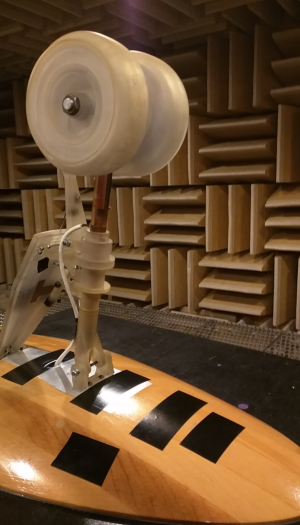
\includegraphics[width=\linewidth]{figures/model1a}
\caption{Baseline 1}
\label{fig:mod1a}
\end{subfigure}
\hspace*{\fill} % separation between the subfigures
\begin{subfigure}{0.45\textwidth}
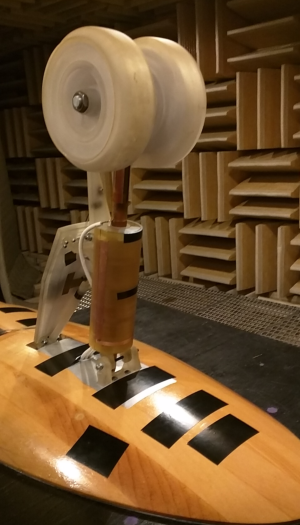
\includegraphics[width=\linewidth]{figures/model1b}
\caption{Baseline 2}
\label{fig:mod1b}
\end{subfigure}
\caption{ND G550 model with and without plasma fairing installed.}
\end{center}
\end{figure}

\section{Notre Dame G550 Nose Landing Gear Model}
Acoustic measurement for two baseline landing gear model configurations were performed. The first, designated Baseline 1, consisted of the ND G550 model without the plasma fairing installed, which is shown in the photograph of Figure \ref{fig:mod1a}. The second, designated Baseline 2, involved the ND G550 model retrofitted with a plasma fairing assembly in order to facilitate installation of dielectric barrier discharge (DBD) plasma actuators for flow control. This configuration is shown in the photograph of Figure \ref{fig:mod1b}.

Spanwise plasma actuators were fixed to the $\pm 90^\circ$ locations to ascertain the effects, if any, on the flow. The plasma actuator was constructed using ULTEM dielectric and 1 in exposed and covered copper electrodes. Also, it was operated using a sine wave carrier frequency of 1 kHz operating at 40 kV peak-to-peak voltage.

\section{Microphone Measurements}
A polar array of omnidirectional microphones was used to acquire far field noise level spectra along the length of the AWT test section. It consists of a 1/2-in ACO Model 7046 electret microphone with companion 4012 preamplifier and PS9200 power supply. A schematic illustrating the array is shown in Figure \ref{fig:array}. Additionally, the array configuration relative to the G550 model is shown in the photograph of Figure \ref{fig:arraypic}. The microphone is mounted using a microphone stand so as to protrude from an acoustically treated rail by approximately 13 in (0.330 m). The total range of acoustic source-to-microphone angle spanned by the polar array is approximately $30^\circ \leq \theta \leq 150^\circ$ as referenced from the upper torque arm of the model in the downstream flow direction. As shown in Figure \ref{fig:arraypic}, the polar array is situated along the length of the free jet test section and positioned at the same height as the upper torque arm of the model, with the plane of the microphone located approximately 59 in (1.50 m) from the test section centerline.

\begin{figure}
	\begin{center}
		\centerline{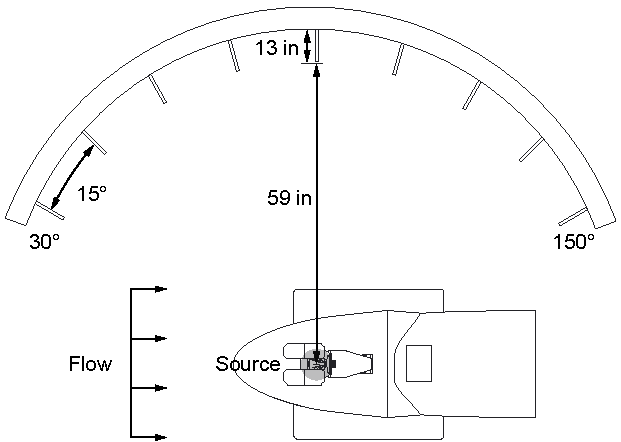
\includegraphics[scale=1.2]{figures/array_schematic}}
		\caption{Schematic of the polar array.}
		\label{fig:array}
	\end{center}
\end{figure}

\begin{figure}
	\begin{center}
		\centerline{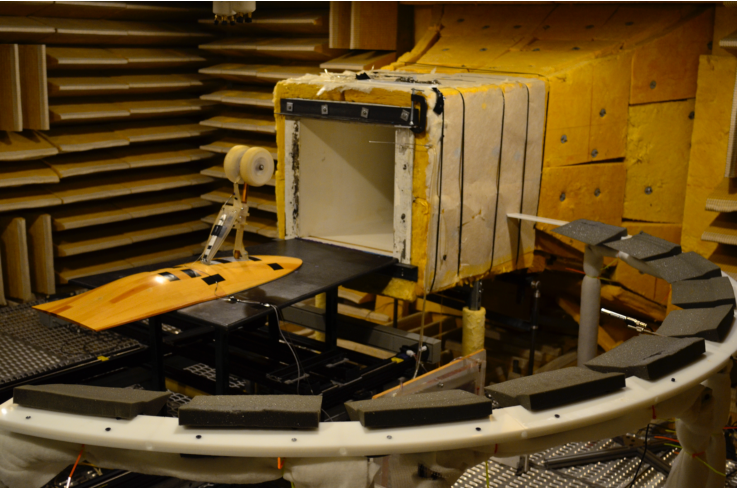
\includegraphics[scale=1.0]{figures/arraypic}}
		\caption{Photograph of the polar array installed in the ND AWT.}
		\label{fig:arraypic}
	\end{center}
\end{figure}

\section{Flow Visualization}
A commercial time-resolved PIV system comprising a Litron Nd:YLF ($\lambda =$ 527 nm) dual-cavity laser and Photron SA1 high-speed camera (12 bit, maximum resolution 1280 x 800 pixels) was utilized. This system was operated in single-frame mode at a repetition rate of 2k frames per second (fps). Images were acquired with a spatial resolution of 1020 x 1020 pixels. During each run, N = 2k images were recorded. A 60 mm Nikon Nikkor Micro lens was fitted and oriented orthogonal and $45^\circ$ to the flow (to resolve region between main strut and door).

Continuous DEHS fog consisting of nominally 1-mm-diameter droplets generated by a TSI six-jet particle atomizer were introduced upstream of the wind-tunnel inlet contraction. The Nd:YLF laser was used to illuminate the fog in a spanwise planes shown in Figure \ref{fig:laserplane}. Flow visualization was performed with baseline 1, 2, and plasma on, in order to assess the global influence on the wake interaction with the main strut and door. 

\section{Data Acquisition}
For microphone data acquisition, a National Instruments USB-6343 DAQ was used, yielding a total of 45 available channels with 48-bit ADC. The sampling parameters for the microphone data acquisition are listed in Table \ref{tab:data}.

\begin{table}
 \setlength{\capwidth}{0.8\textwidth}
\begin{center}
\caption{Data acquisition parameters.}
\label{tab:data}
\begin{tabular}{cccccccc}\toprule
\parbox{0.1\linewidth}{\centering Sensors} & 
\parbox{0.12\linewidth}{\centering Sampling Rate (Hz)} & 
\parbox{0.1\linewidth}{\centering $\frac{Samples} {block}$} & 
\parbox{0.11\linewidth}{\centering Window Function} & 
\parbox{0.1\linewidth}{\centering Overlap (\%)} & 
\parbox{0.1\linewidth}{\centering $N_{blocks}$} & 
\parbox{0.1\linewidth}{\centering $N_{averages}$} & 
\parbox{0.11\linewidth}{\centering Acquisition Time (s)} \\ \midrule
ACO & 65,536 & 2048 & Hanning & 0 & 960 & 960 & 30 \\ \bottomrule
\end{tabular}
\end{center}
\end{table}

\section{Current Results}

\subsection{Wind Tunnel Background Noise Characterization}
It was deemed important to establish that the background noise levels in the ND AWT were sufficiently below that of the ND G550 model. To that end, measurement of noise levels for both Baseline 1 and Baseline 2 G550 configurations were compared with those obtained with the AWT tunnel running empty. Figure \ref{fig:empty} presents a representative comparison of 1/3-octave band sound pressure level (SPL) spectra obtained for the Baseline 1 configurations and the empty tunnel. The figure clearly shows that the background empty tunnel noise level is several orders of magnitude below that of the ND G550, so that the effects of plasma flow control on noise production will be detectable in this facility.

\begin{figure}
	\begin{center}
		\centerline{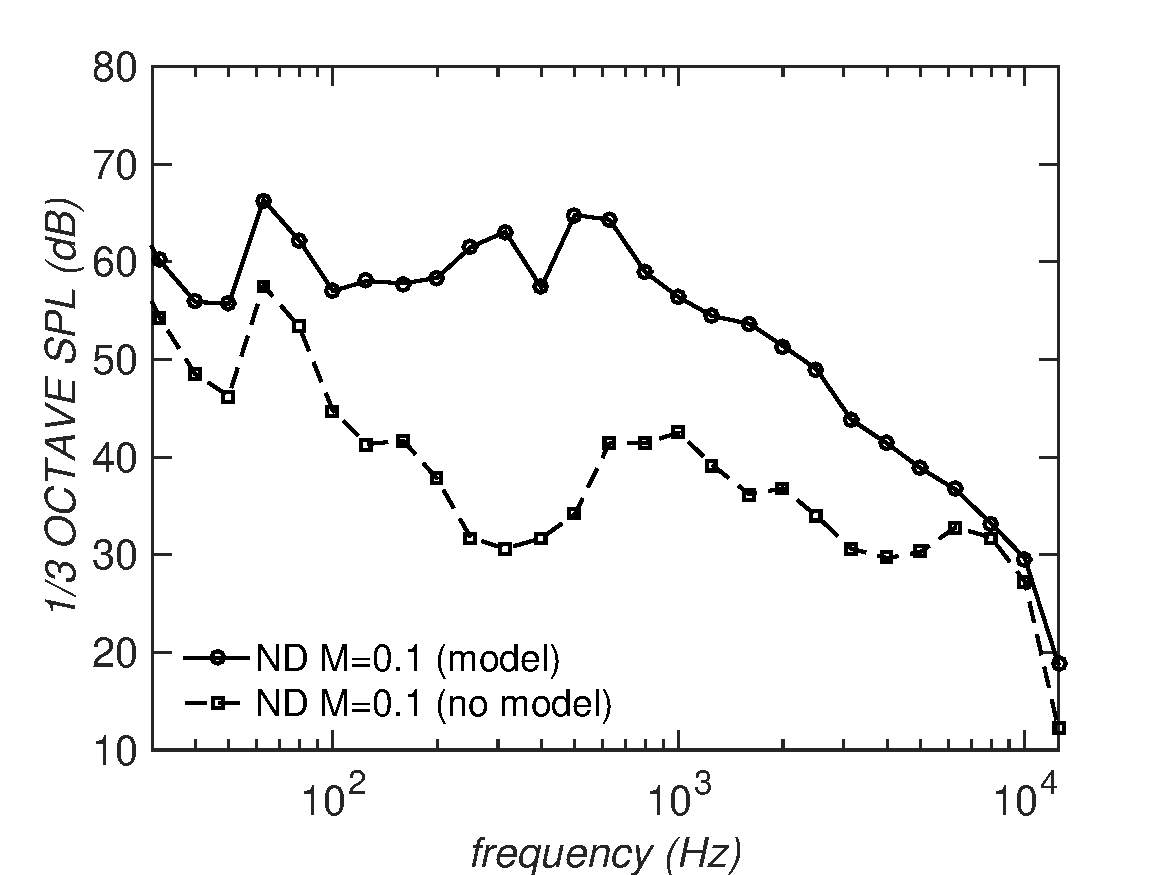
\includegraphics[scale=0.7]{figures/mic_empty}}
		\caption{Representative far field noise level with and without Baseline 1 model installed at $\theta = 90^\circ$}
		\label{fig:empty}
	\end{center}
\end{figure}

\subsection{Far field check}
This section describes a procedure for verifying the far field assumption for microphone measurements.
For a microphone measurement to be classified as far field, the microphone-to-source distance must be greater than the acoustic wavelength. To check this a relation can be made between power spectral density, $PSD$, and microphone-to-source distance, $d$. Recall from equation \ref{eq:pflux} that $p' \approx 1/d$, therefore, it follows that $PSD \approx 1/d$. Combining this relation at $d =$ 48 in and $d =$ 59 yields,

\begin{equation}
\frac{PSD_1}{PSD_2} \approx \frac{d_2}{d_1} \approx 1.23.
\end{equation}

The $PSDs$ at both of these locations is plotted along with a reference line at 1.23 in Figure \ref{fig:far}. The measured microphone data exhibits oscillations about the theoretical value of 1.23. The average of the oscillations collapses to the theoretical value if one excludes frequencies below 100 Hz. This suggests that to resolve frequencies below 100 Hz larger values for $d$ are necessary. Previous experiments have reinforced that this lower limit on acoustic measurements is acceptable.
 
\begin{figure}
	\begin{center}
		\centerline{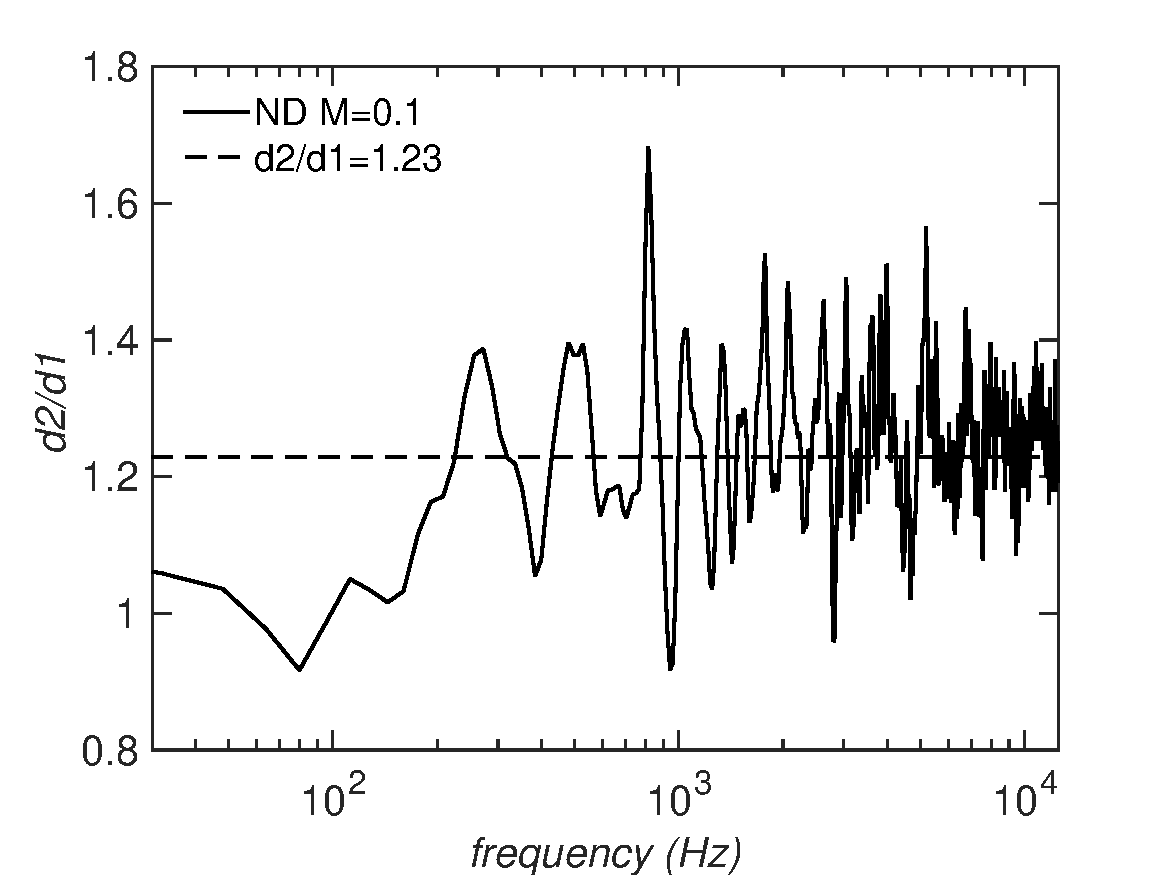
\includegraphics[scale=0.7]{figures/mic_far}}
		\caption{Far field measurement analysis for $d =$ 48 in and $d =$ 59 in at $\theta = 90^\circ$}.
		\label{fig:far}
	\end{center}
\end{figure}

\subsection{Comparison with UFAFF Measurements}
To match the numerical simulations being performed concurrently in this study, the far field microphone distance $d$, was 72 in (1.83 m) array-to-model and 59 in (1.50 m) microphone-to-model. However, previous studies conducted at the University of Florida Anechoic Flow Facility (UFAFF) on the NASA G550 model were performed at a source-to-microphone distance of 48 in. In order to form a basis for comparison with acoustic results from that study, 1/3-octave band SPL spectra were obtained with the ND Baseline 1 model in the ND AWT for a source-to-microphone distance of 48 in (1.22 m). Even after accounting for the source-to-microphone distance disparity, the UFAFF experiments were performed at a freestream Mach number $M_\infty =$ 0.189 and the Notre Dame experiments were performed at $M_\infty=$ 0.1. The effect of disparate Mach numbers on the SPL can be accounted for by scaling the Notre Dame results via the relation, 

\begin{equation}
SPL_2 = SPL_1 - 10 \log \left( \frac{M_1}{M_2} \right)^6,
\end{equation}

where $SPL_1$ and $M_1$ denote the ND AWT experimental values, $M_2$ denotes the UFAFF test Mach number (0.189) and $SPL_2$ represents the ND AWT sound pressure level values corrected for Mach number. Figure \ref{fig:farfield} compares 1/3-octave band SPL spectra obtained in both facilities for the case of $\theta = 90^\circ$. In this plot the frequency is expressed in terms of Strouhal number, $St_D = f D / U_\infty$, where length scale $D$ is the shock strut diameter upstream of the torque arm and $U_\infty$ is the freestream velocity.
There is good collapse of the NASA G550 and ND G550 data from $0.3 \leq St_D \leq 0.6$. Below this range there is about 4-5 dB difference before the 100 Hz AWT cutoff frequency. Above this range there is significant discrepancy. The NASA G550 model is characterized by a peak near $St_D=$ 3 and spectral roll-off above this peak. The ND G550 model lacks this high frequency content. The components of the ND G550 model are mostly fabricated from SLA plastic, while the NASA G550 consists of mostly aluminum and carbon fiber. To compensate for the differences in tensile strength, thickness was added to several components of the ND G550 model as shown in the CAD images in Figure \ref{fig:cad}. Additionally, it was necessary to construct most of the ND G550 model from plastic to facilitate the retrofitting of plasma actuators. It is possible, but by no means certain that these design modifications may play a roll in the observed differences in noise spectra.

\begin{figure}
	\begin{center}
		\centerline{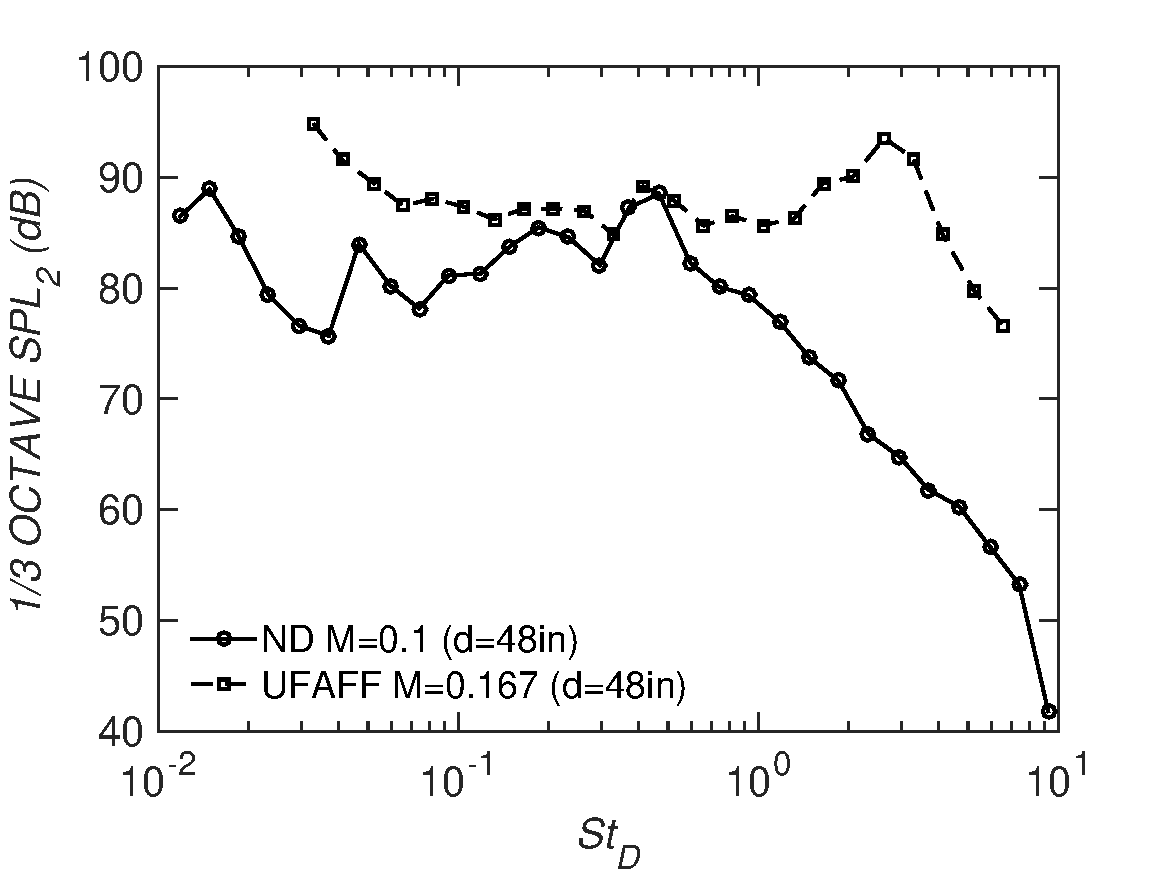
\includegraphics[scale=0.7]{figures/nd_ufaff}}
		\caption{Comparison of far field noise level at UFAFF and ND AWT facilities at $\theta = 90^\circ$}
		\label{fig:farfield}
	\end{center}
\end{figure}

\begin{figure}
\begin{center}
\begin{subfigure}{0.45\textwidth}
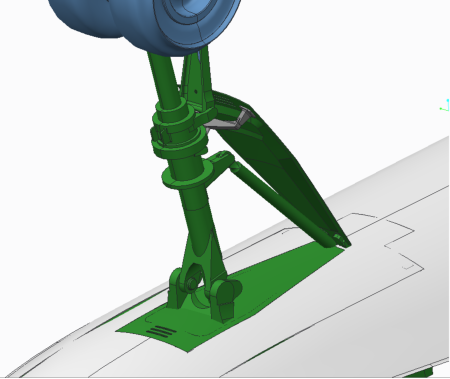
\includegraphics[width=\linewidth]{figures/nasag550}
\caption{NASA G550}
\label{fig:nasag550}
\end{subfigure}
\hspace*{\fill} % separation between the subfigures
\begin{subfigure}{0.45\textwidth}
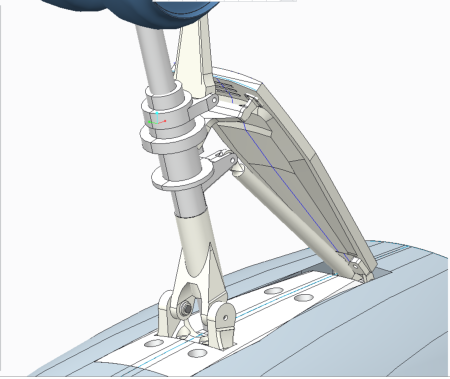
\includegraphics[width=\linewidth]{figures/ndg550}
\caption{ND G550}
\label{fig:ndg550}
\end{subfigure}
\caption{Comparison of design of the NASA G550 and ND G550 model geometries.}
\label{fig:cad}
\end{center}
\end{figure}

\subsection{Effects of Tripping}
Previous work on the NASA G550 Nose Landing Gear (NASA G550) involved application of serrated transition strips that were applied along the length of the shock strut in order to create a turbulent boundary layer prior to separation. For consistency with this previous work, the influence of similar aerodynamic trips was explored on the ND G550 Baseline 1 model. A distributed roughness element made of standard diving board tape was fixed to the shock strut. Sample results comparing 1/3-octave band SPL spectra for the tripped and untripped cases are presented in Figure \ref{fig:trip}. This figure shows that there was very little influence of the trip on radiated noise. Since a trip would restrict the optimum placement of the plasma actuators, it was omitted from the model and the acoustic results that follow were obtained without tripping unless otherwise indicated.

\begin{figure}
	\begin{center}
		\centerline{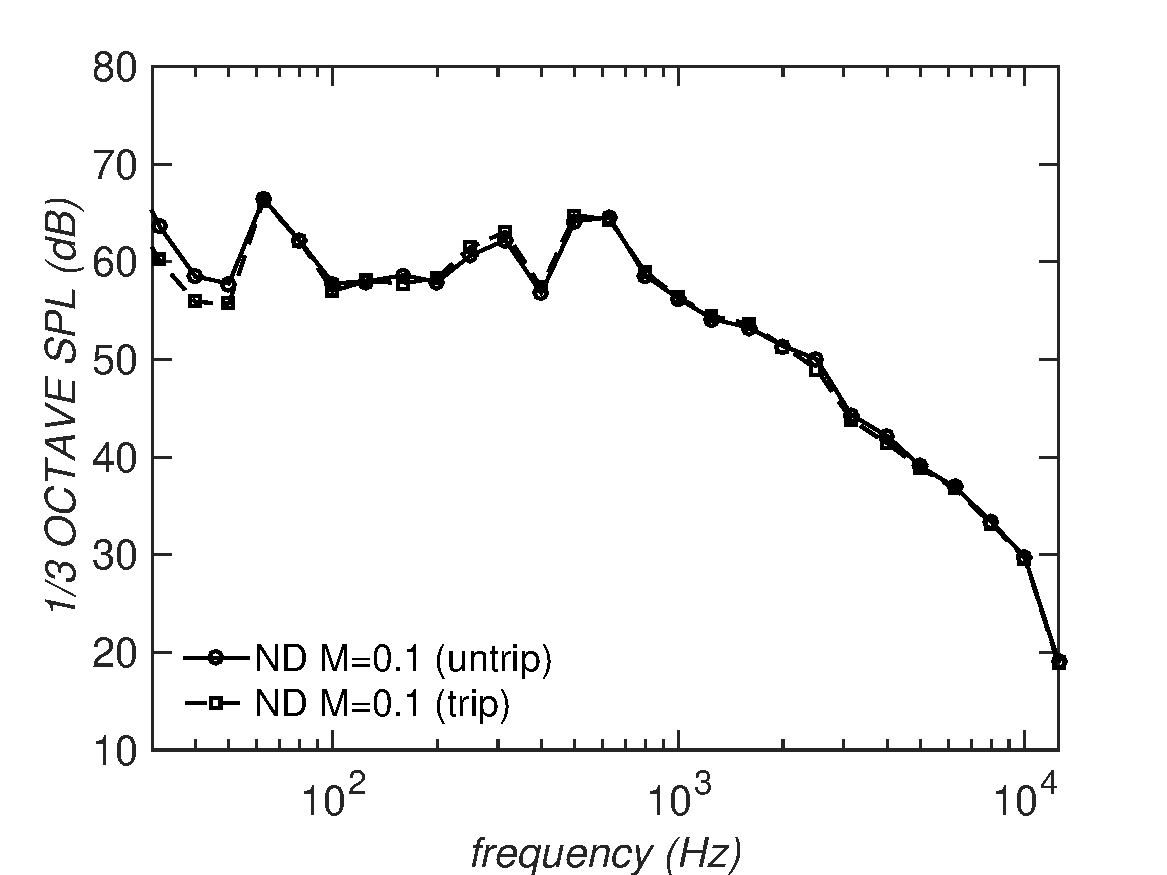
\includegraphics[scale=0.7]{figures/mic_trip}}
		\caption{Comparison of far field noise level with and without the presence of a trip at $\theta = 90^\circ$}
		\label{fig:trip}
	\end{center}
\end{figure}

\subsection{Preliminary Acoustic Assesment}
Three key locations on the polar array were selected for microphone measurements. This allowed several plasma actuator configurations to be tested expediently to quickly assess noise reduction. Four plasma actuator configurations were utilized: 1) Baseline 1, 2) Baseline 2, 3) Sine 40 kV (Two-sides), 4) Sine 40 kV (One-side). The effect of the fairing geometry is shown with 1) and 2), while 3) and 4) demonstrate the effects of plasma actuation. The maximum peak-to-peak voltage attainable with the ULTEM dielectric was 40 kV before signs of dielectric failure were observed. In subsequent experiments, a dielectric that is less susceptible to failure, such as quartz, is recommended. 

The 1/3-octave band SPL spectra for the aforementioned actuator configurations are given in Figure \ref{fig:octave}. Recall from Figure \ref{fig:mic_empty}, that the left most peak is below the 100 Hz cutoff frequency and is most likely due to fan noise inherent to the facility. The acoustic signature at each location is characterized by two peaks at approximately $300$ Hz and $500$ Hz of varying magnitude. Most of the change caused by the plasma fairing occurs around these frequencies, with the exception of a slight increase in frequency due to the self-noise of the plasma actuators for $6 \leq f \leq 12.5$. 

The Overall Sound Pressure Level (OASPL) is calculated by integrating the power spectral density from $100 \leq f \leq 1000$ Hz. This range was selected to eliminate te effect of plasma self-noise which is operated at a carrier frequency of 1000 Hz. OASPL at each location, $\theta = 45^\circ, 90^\circ, 135^\circ$, is given in Figure \ref{fig:polar}. There is a slight decrease for the Baseline 2 and sine 40 kV one-side cases at $\theta = 135^\circ$ of 0.12 dB and 0.13 dB, respectively. Also, the plasma actuation actually increased the noise at each location with the exception of the sine 40 kV one-sided case at $\theta = 135^\circ$. 

To better understand the perplexing results of the acoustic measurements, flow visualization was performed to resolve the change to the global flow field and the effects on the main strut and door wake interaction. The results are given in Figure \ref{fig:flowvis}.  

%\begin{figure}
%\centering
%\begin{subfigure}{0.32\textwidth}
%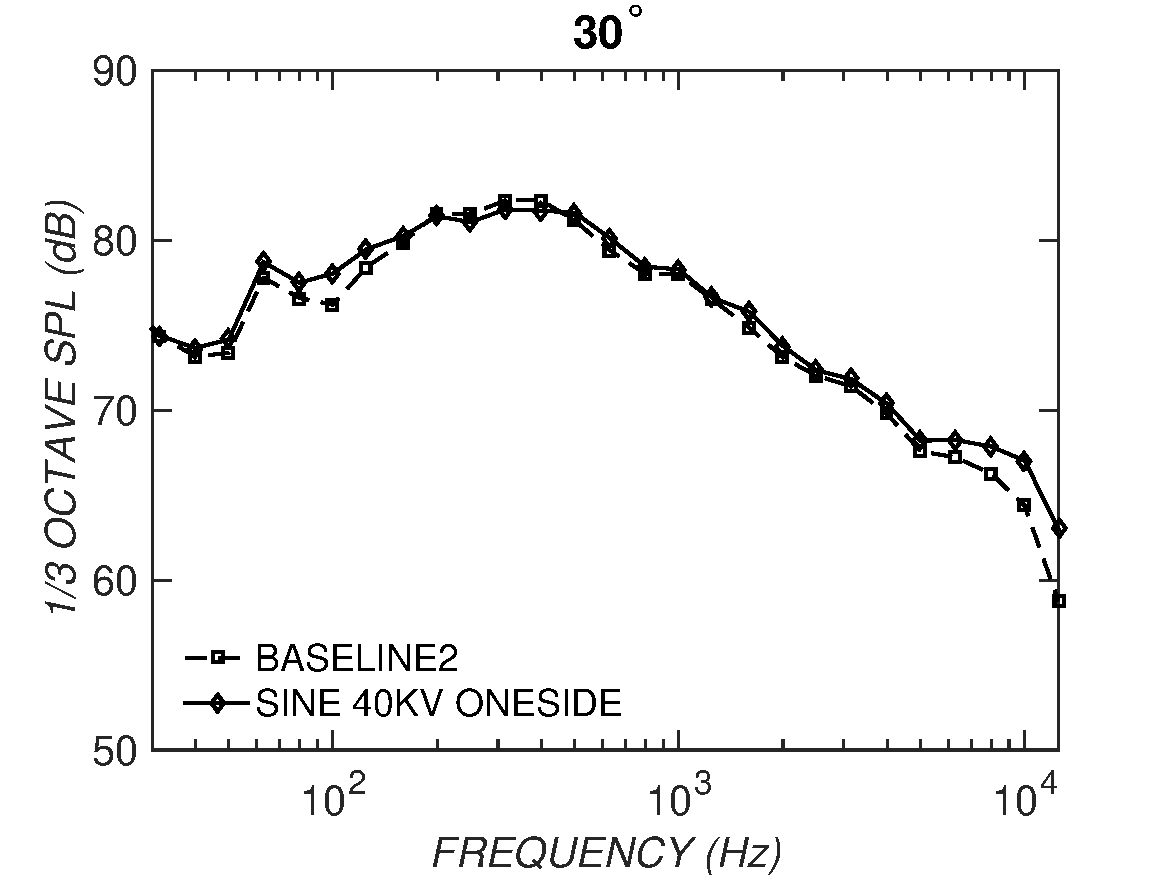
\includegraphics[width=\linewidth]{figures/octave302}
%\caption{$\theta=30^\circ$}
%\label{fig:octave302}
%\end{subfigure}%
%\hspace*{\fill} % separation between the subfigures
%\begin{subfigure}{0.32\textwidth}
%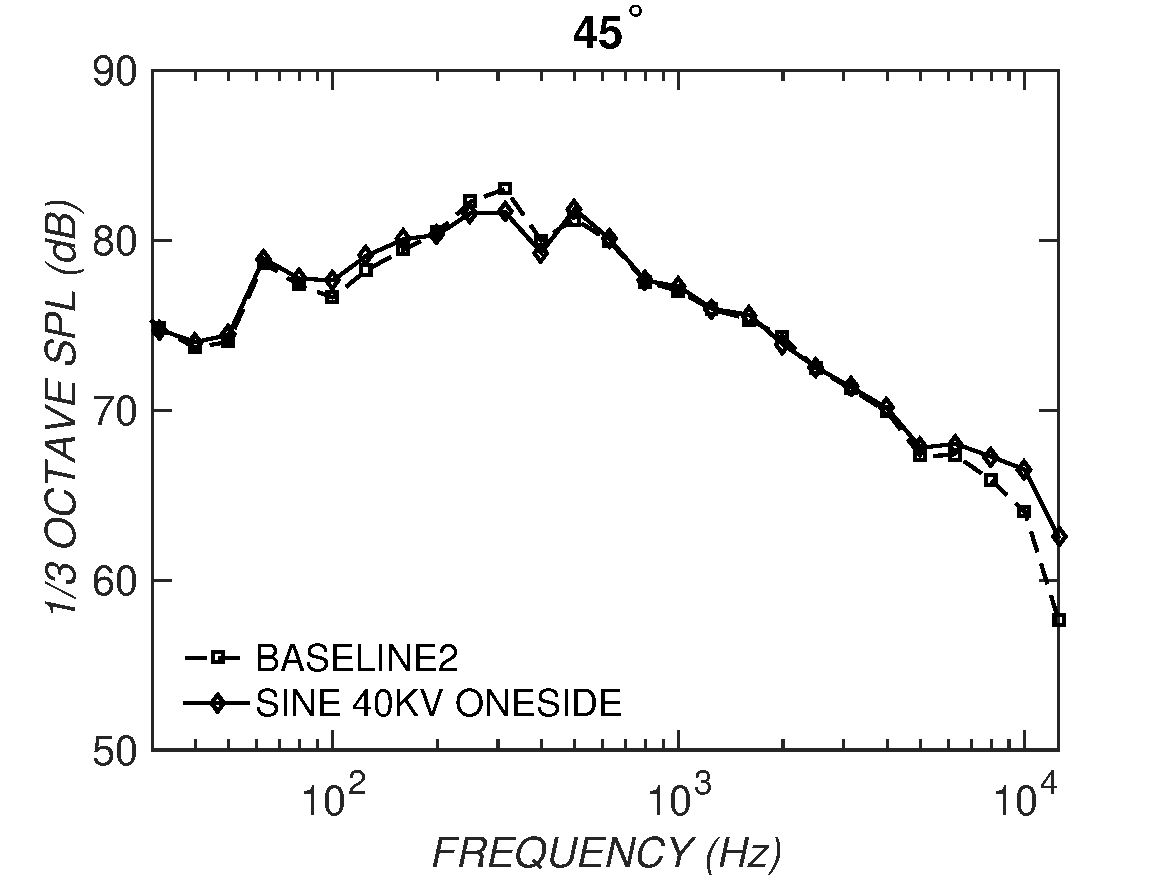
\includegraphics[width=\linewidth]{figures/octave452}
%\caption{$\theta=45^\circ$}
%\label{fig:octave452}
%\end{subfigure}%
%\hspace*{\fill} % separation between the subfigures
%\begin{subfigure}{0.32\textwidth}
%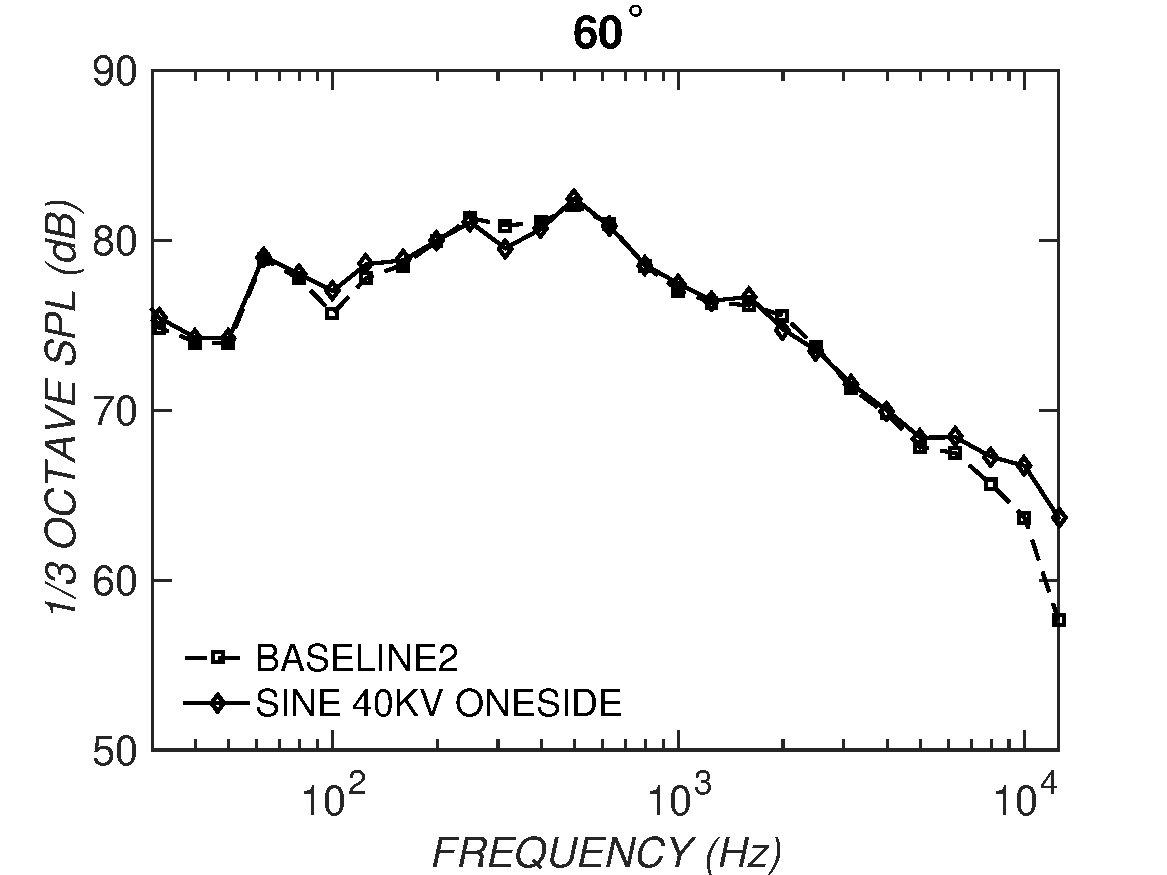
\includegraphics[width=\linewidth]{figures/octave602}
%\caption{$\theta=60^\circ$}
%\label{fig:octave602}
%\end{subfigure}%
%
%\begin{subfigure}{0.32\textwidth}
%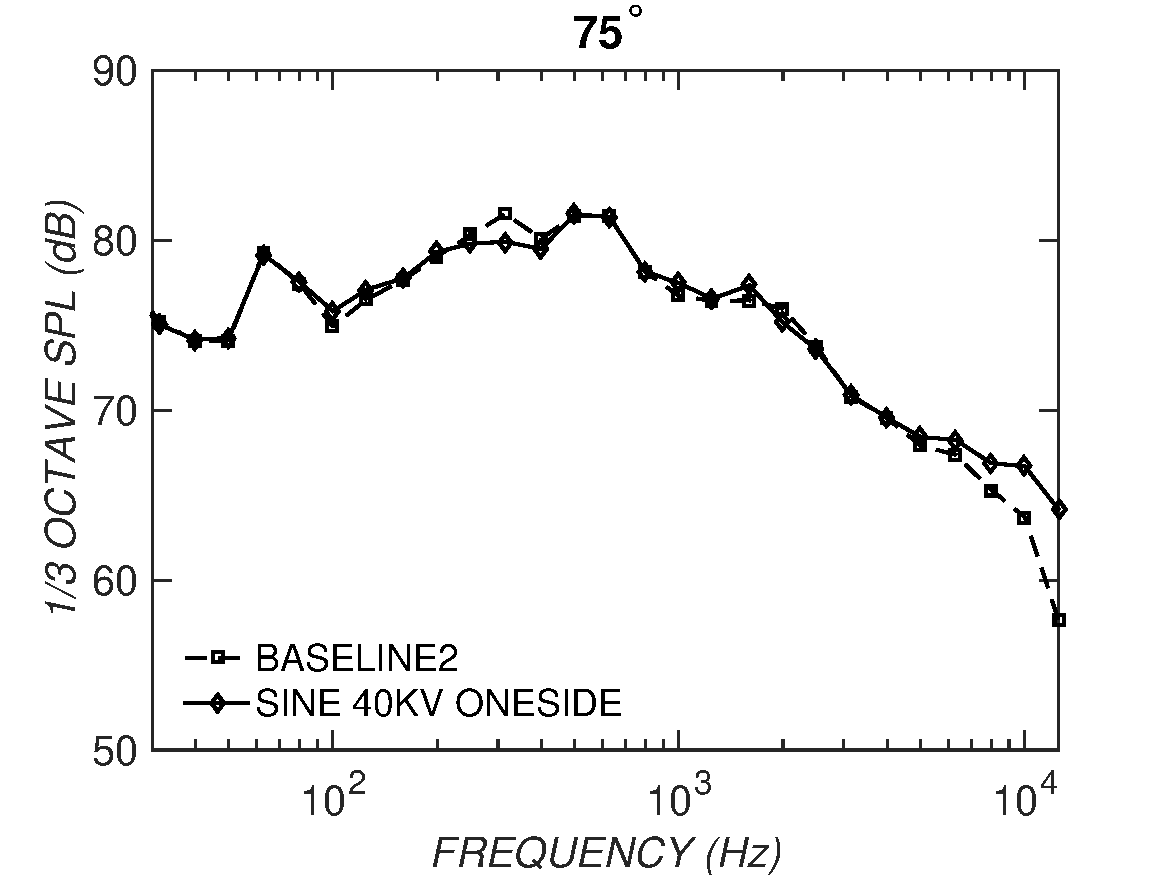
\includegraphics[width=\linewidth]{figures/octave752}
%\caption{$\theta=75^\circ$}
%\label{fig:octave752}
%\end{subfigure}%
%\hspace*{\fill} % separation between the subfigures
%\begin{subfigure}{0.32\textwidth}
%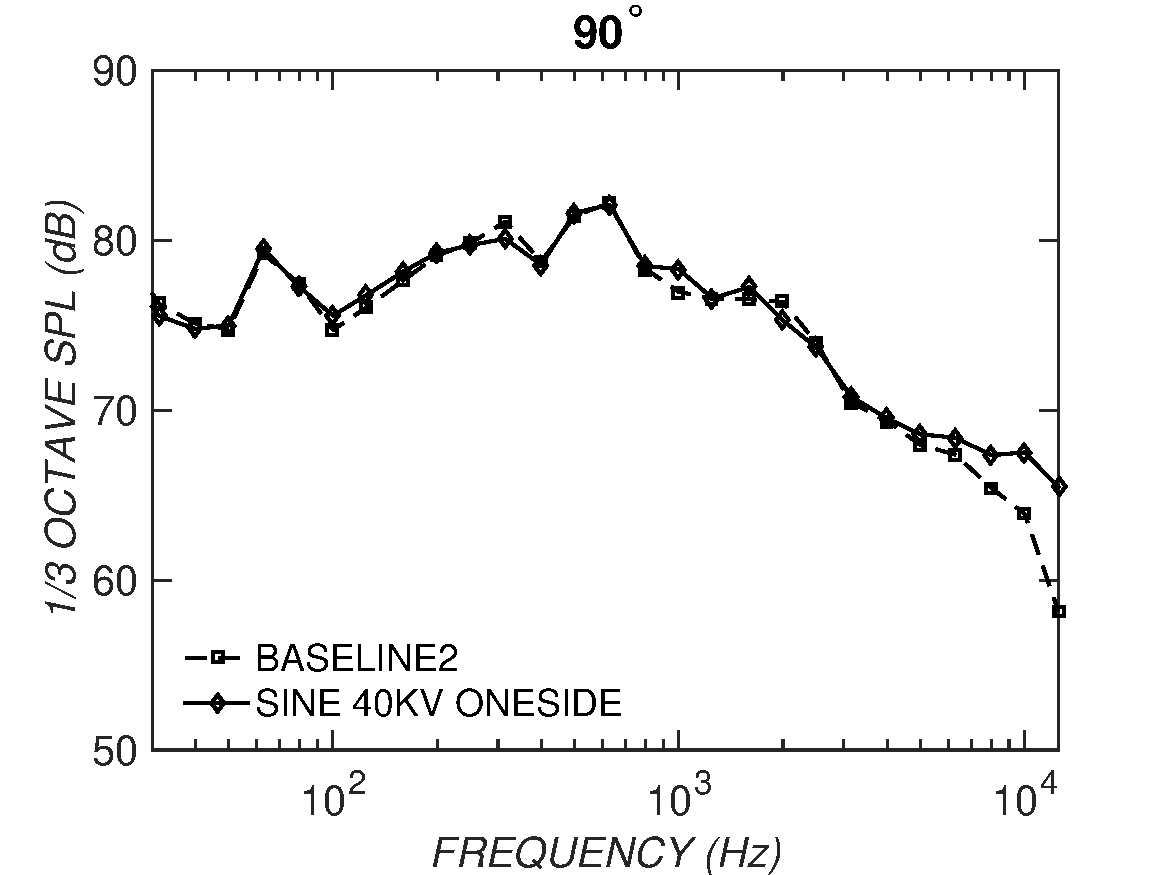
\includegraphics[width=\linewidth]{figures/octave902}
%\caption{$\theta=90^\circ$}
%\label{fig:octave902}
%\end{subfigure}
%\hspace*{\fill} % separation between the subfigures
%\begin{subfigure}{0.32\textwidth}
%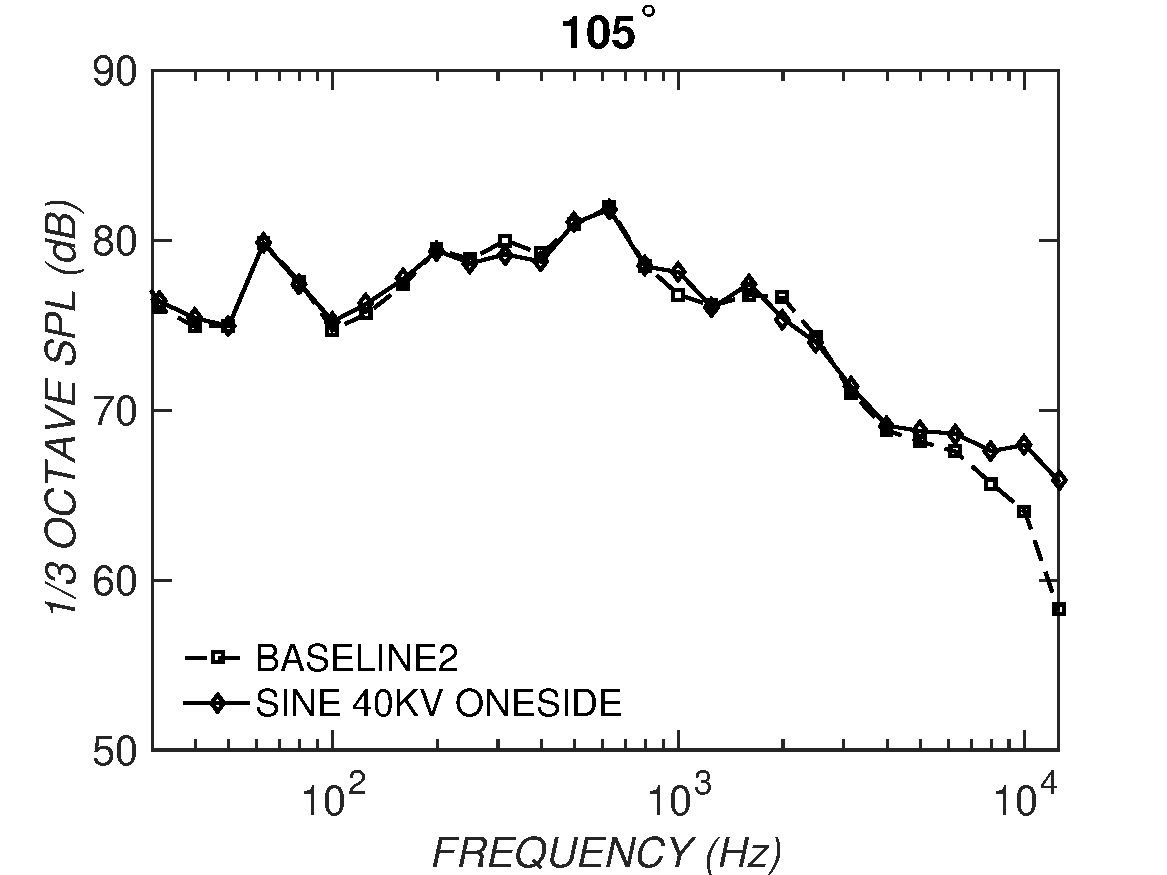
\includegraphics[width=\linewidth]{figures/octave1052}
%\caption{$\theta=105^\circ$}
%\label{fig:octave1052}
%\end{subfigure}
%
%\begin{subfigure}{0.32\textwidth}
%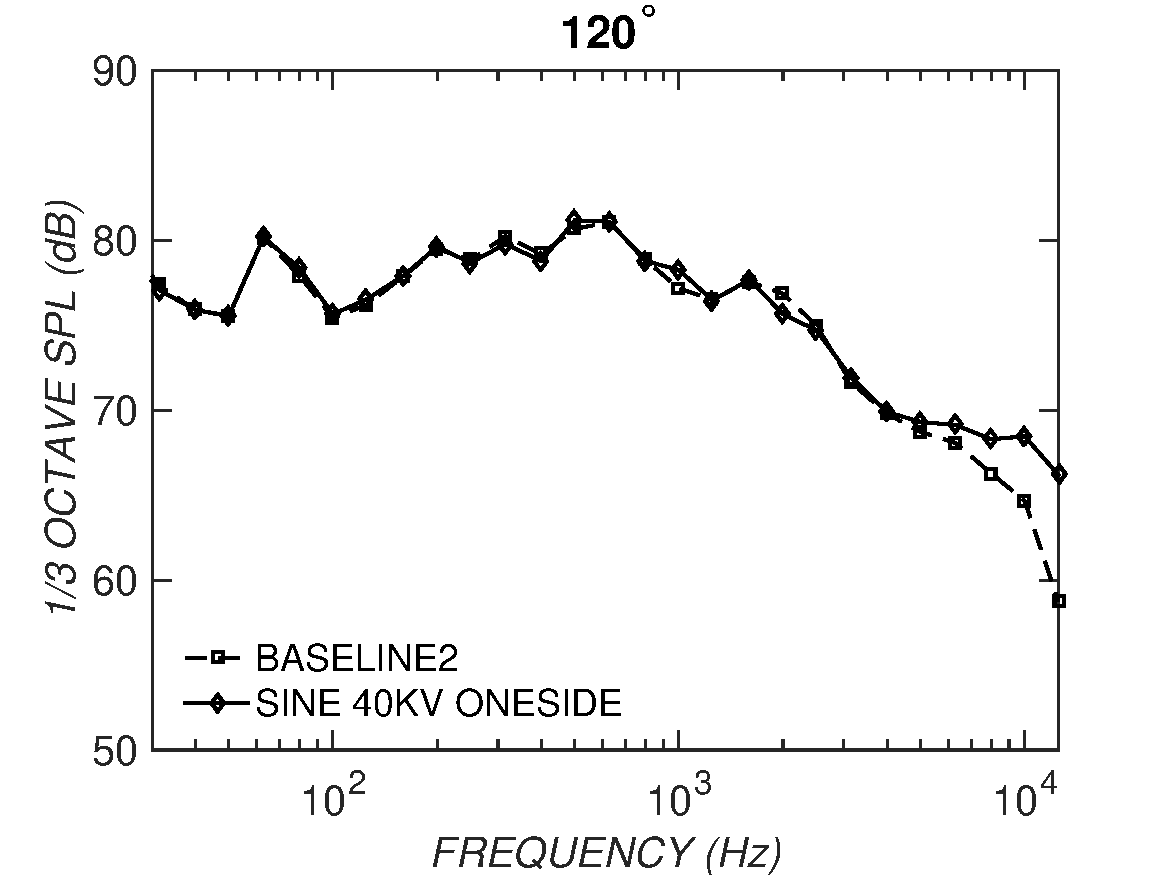
\includegraphics[width=\linewidth]{figures/octave1202}
%\caption{$\theta=120^\circ$}
%\label{fig:octave1202}
%\end{subfigure}
%\hspace*{\fill} % separation between the subfigures
%\begin{subfigure}{0.32\textwidth}
%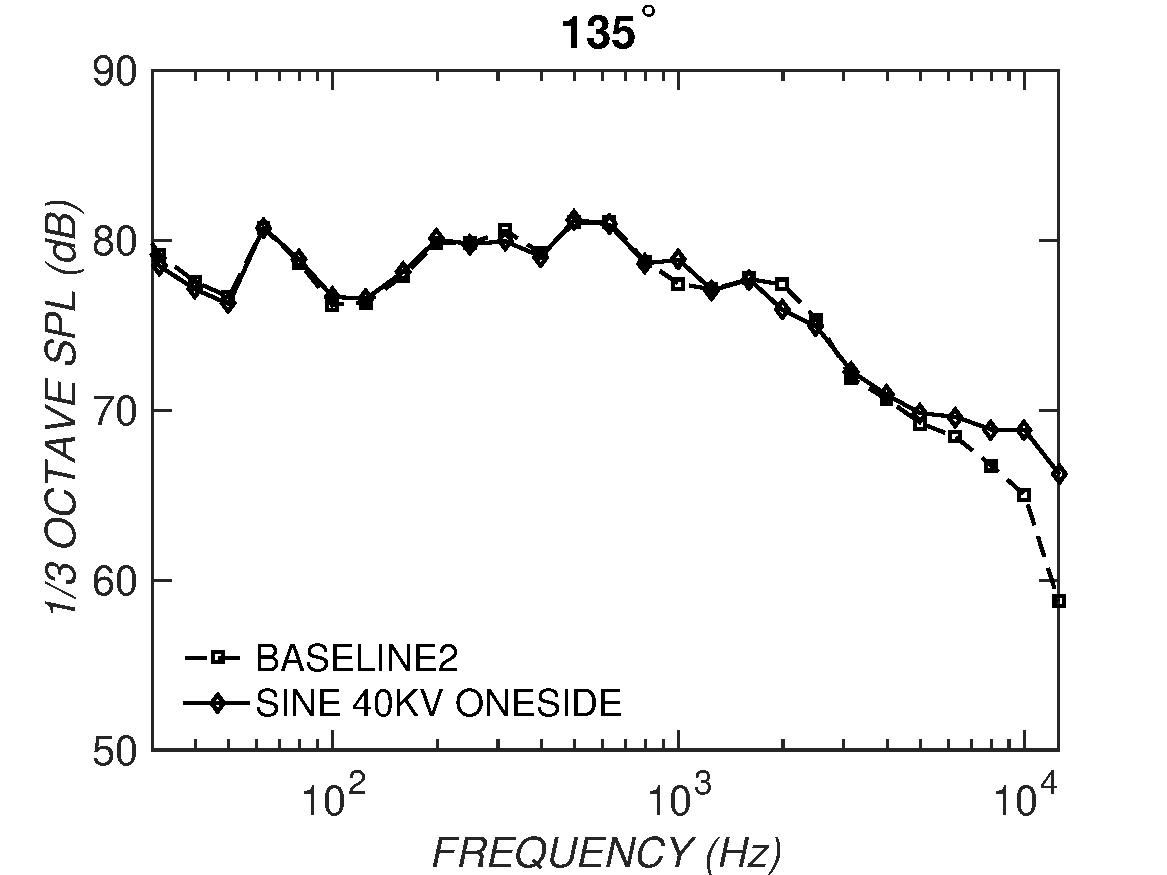
\includegraphics[width=\linewidth]{figures/octave1352}
%\caption{$\theta=135^\circ$}
%\label{fig:octave1352}
%\end{subfigure}
%\hspace*{\fill} % separation between the subfigures
%\begin{subfigure}{0.32\textwidth}
%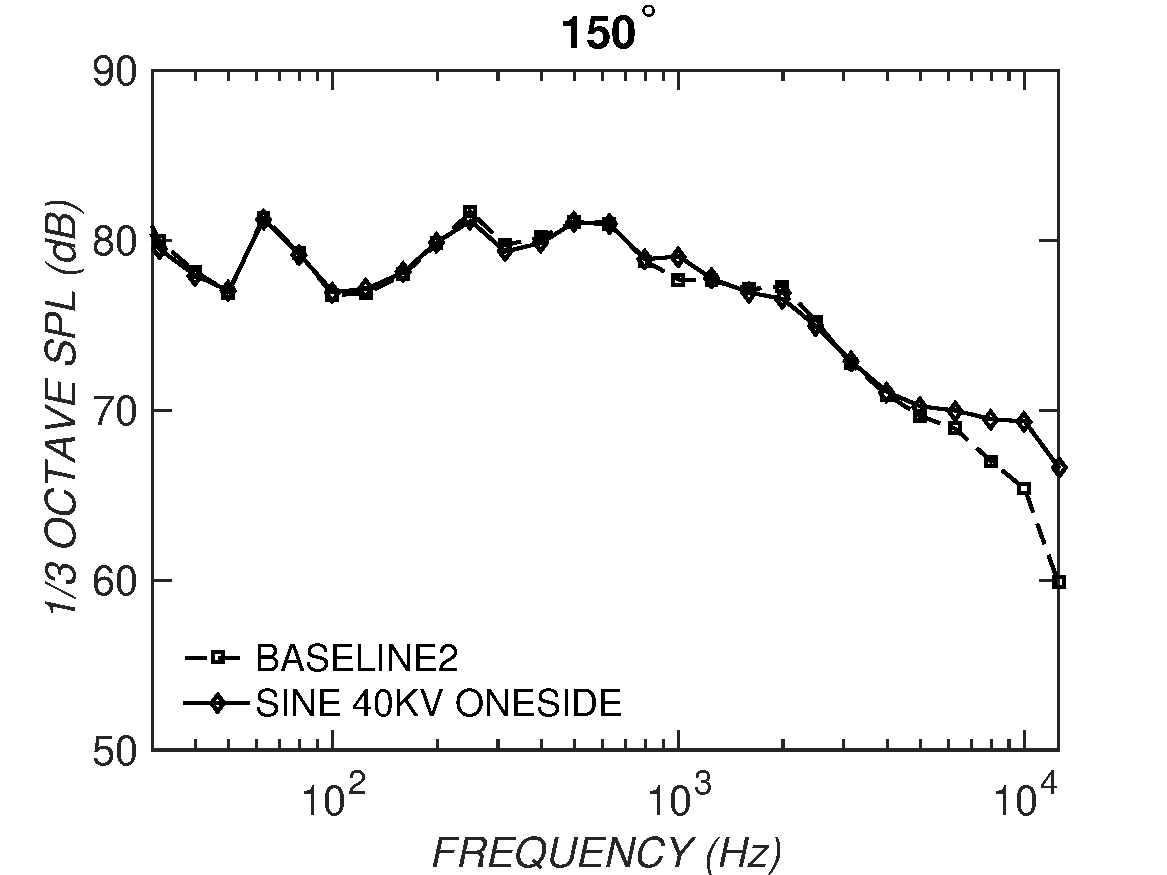
\includegraphics[width=\linewidth]{figures/octave1502}
%\caption{$\theta=150^\circ$}
%\label{fig:octave1502}
%\end{subfigure}
%
%\caption{1/3-octave band SPL}
%\label{fig:octave2}
%\end{figure}

\begin{figure}
\begin{center}
\begin{subfigure}{0.5\textwidth}
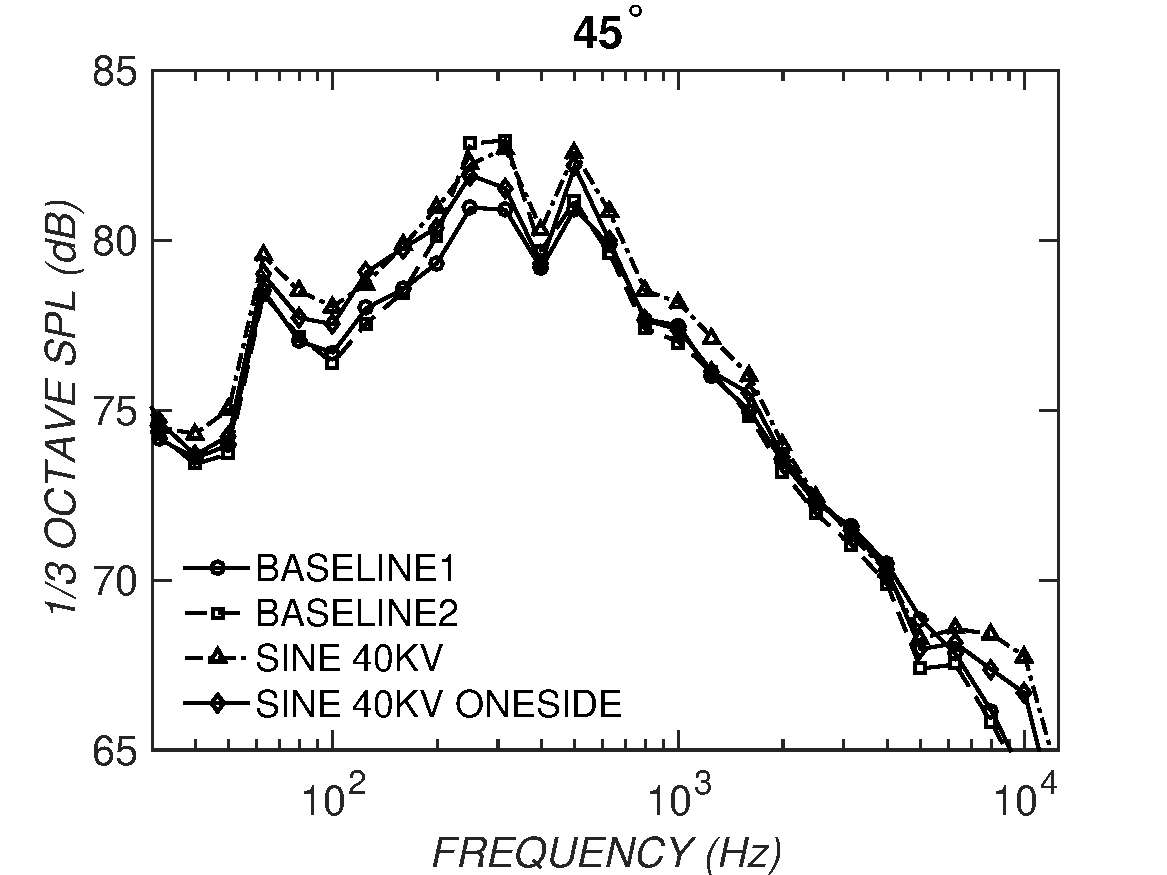
\includegraphics[width=\linewidth]{figures/octave45}
\caption{$\theta=45^\circ$}
\label{fig:octave45}
\end{subfigure}

\hspace*{\fill} % separation between the subfigures

\begin{subfigure}{0.5\textwidth}
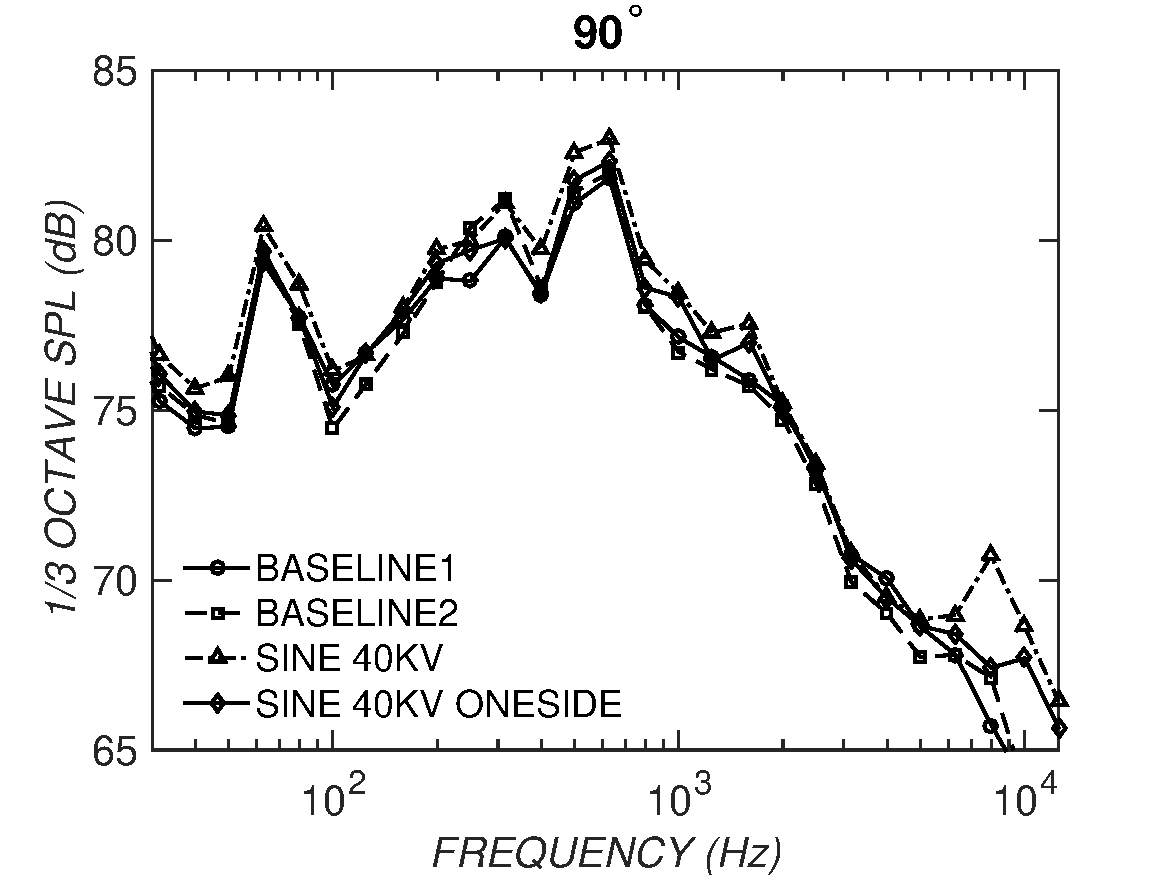
\includegraphics[width=\linewidth]{figures/octave90}
\caption{$\theta=90^\circ$}
\label{fig:octave90}
\end{subfigure}

\hspace*{\fill} % separation between the subfigures

\begin{subfigure}{0.5\textwidth}
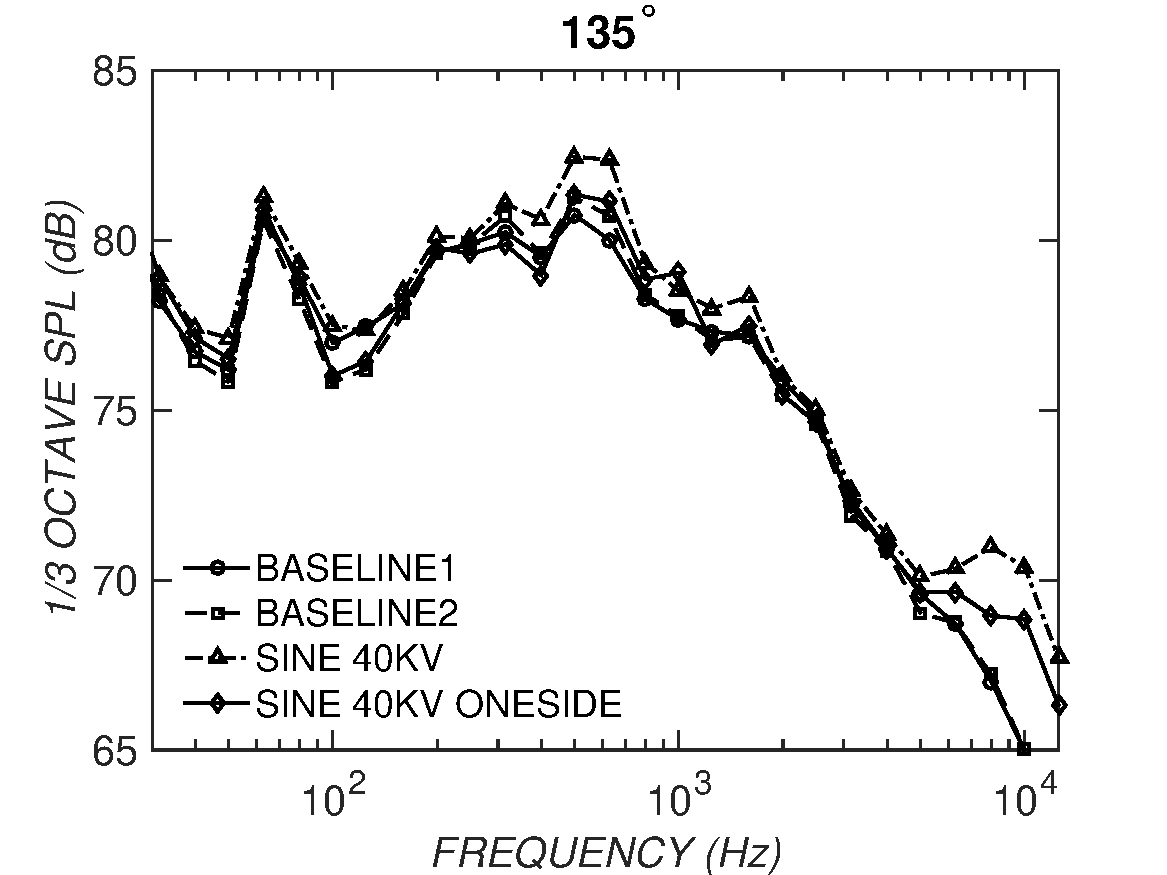
\includegraphics[width=\linewidth]{figures/octave135}
\caption{$\theta=135^\circ$}
\label{fig:octave135}
\end{subfigure}

\caption{1/3-octave band SPL}
\label{fig:octave}
\end{center}
\end{figure}

\begin{figure}
	\begin{center}
		\centerline{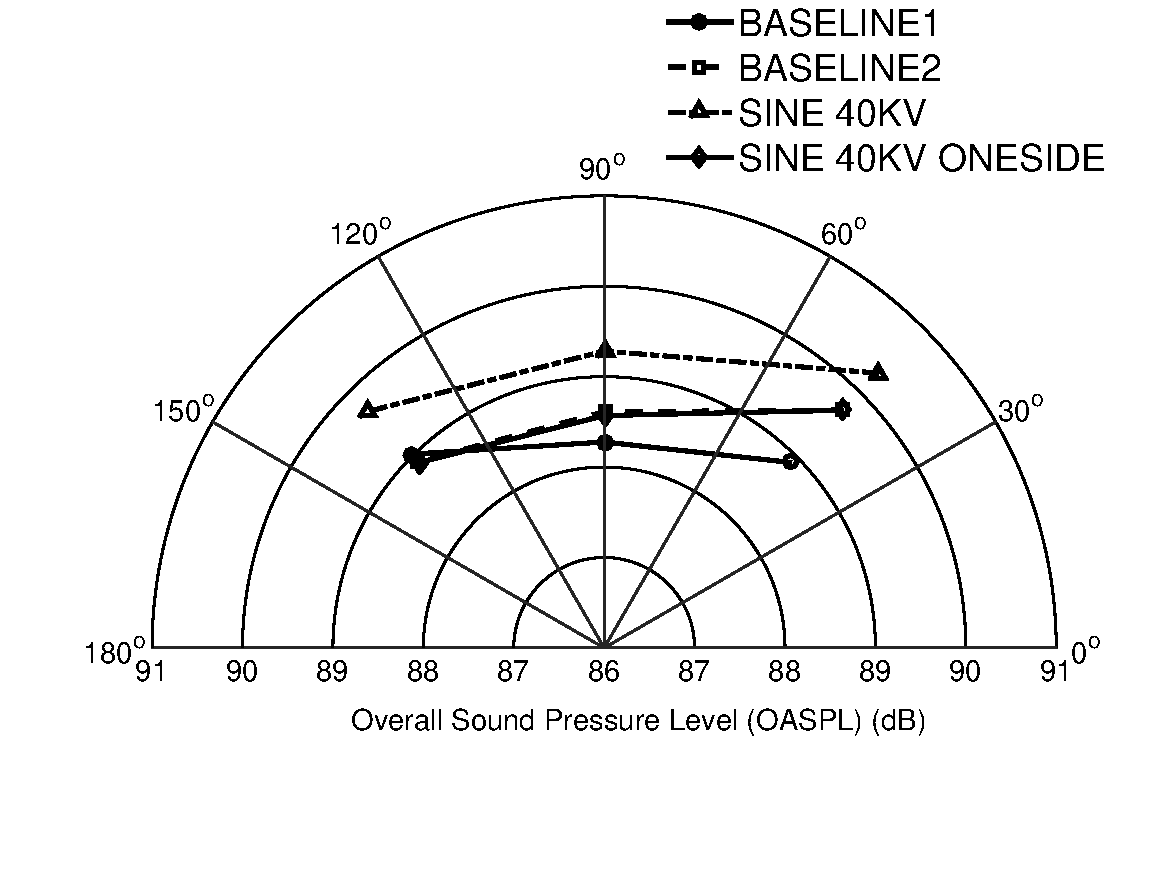
\includegraphics[scale=0.7]{figures/polar_plot4}}
		\caption{Polar plot}
		\label{fig:polar}
	\end{center}
\end{figure}

\begin{figure}
	\begin{center}
		\centerline{\includegraphics[scale=0.7]{figures/flowvis}}
		\caption{Landing Gear Flow Visualization}
		\label{fig:flowvis}
	\end{center}
\end{figure}




%In preparation for reading this dissertation, I would highly recommend
%reading some of the other material available on
%Gnus~\citep{gnus98:_gerry_ganst,greenfield96:_gettin_know_gnu}.  They
%are very well written and will give you a fuller understanding of
%Gnus.
%
%Gnus are frequently mistakes for squirrels.  They are not squirrels.
%They are Gnus.  Don't call them squirrels, either (unless you have
%food in your hand); they tend to get a bit upset.\footnote{This is
%  frequently mistaken for the chattering and scampering away.  Gnus
%  are actually quite polite; they will leave if they have nothing nice
%  to say, for fear of saying something offensive.}  If you have food
%in your hand, they tend to ignore this insult and accept your food as
%a peace offering.\footnote{Sometimes they'll follow you if you continue
%to refuse to feed them.}

%Table~\ref{tbl:bogus1} shows some feeding frequencies for where Gnus
%like to eat around the Notre Dame campus.  Gnus have work weeks, just
%like humans do, hence the much lower frequencies on weekends.  This
%can lead us to conclude that Gnu weekend shifts are much smaller than
%the normal work-week shifts.  In fact, we can attempt to parametrize the
%sighting frequency, $\mathcal{F}$, by the student population, type of food, and
%day of the week as:
%\begin{equation}
%  \mathcal{F} = \mathcal{F}(p,f,d).
%\end{equation}
%Table~\ref{tbl:bogus2} shows what they
%typically like to eat.
%
%\begin{table}[tpb]
%  \begin{center}
%    \caption{WHERE Gnus LIKE TO EAT \label{tbl:bogus1}}
%    \begin{tabularx}{0.85\textwidth}{lrrrrrrr} \toprule
%      \multicolumn{1}{c}{Location} & Sun & Mon & Tue & Wed & Thu & Fri & Sat \\ \midrule
%      Front of Dome & 1 & 5 & 6 & 5 & 4 & 5 & 1 \\
%      Stonehenge & 2 & 9 & 10 & 12 & 9 & 14 & 2 \\
%      The Rock & 1 & 3 & 4 & 3 & 4 & 3 & 0 \\
%      The ACC & 3 & 4 & 5 & 5 & 5 & 4 & 1 \\
%      Dining Halls & 5 & 14 & 12 & 13 & 14 & 12 & 3 \\
%      Hesburgh Library & 2 & 3 & 5 & 2 & 3 & 4 & 2 \\ \bottomrule
%    \end{tabularx}
%  \end{center}
%\end{table}
%
%\begin{table}[tpb]
%  \setlength{\capwidth}{0.7\textwidth}
%  \begin{center}
%    \caption{WHAT Gnus LIKE TO EAT ON THE NOTRE DAME CAMPUS, LISTED
%      BY AVERAGE NUMBER OF SIGHTINGS PER WEEKDAY
%    \label{tbl:bogus2}
%}
%    \begin{tabular}{lrrrrrrr} \toprule
%      \multicolumn{1}{c}{Food} & Sun & Mon & Tue & Wed & Thu & Fri & Sat \\ \midrule
%      Twinkies & 1 & 5 & 6 & 5 & 4 & 5 & 1 \\
%      Ding Dongs & 2 & 9 & 10 & 12 & 9 & 14 & 2 \\
%      Carrots & 1 & 3 & 4 & 3 & 4 & 3 & 0 \\
%      Lettuce & 3 & 4 & 5 & 5 & 5 & 4 & 1 \\
%      Twizlers & 5 & 14 & 12 & 13 & 14 & 12 & 3 \\
%      Jawbreakers & 2 & 3 & 5 & 2 & 3 & 4 & 2 \\ \bottomrule
%    \end{tabular}
%  \end{center}
%\end{table}
%
%Figure~\ref{fig:bogus3} shows a nice graph of location distributions
%by day of week.  I have no real reason for including it except to show
%that figures work as well.  Did I mention that Gnus are really cool?
%
%\begin{figure}[tpb]
%  \begin{center}
%    \centerline{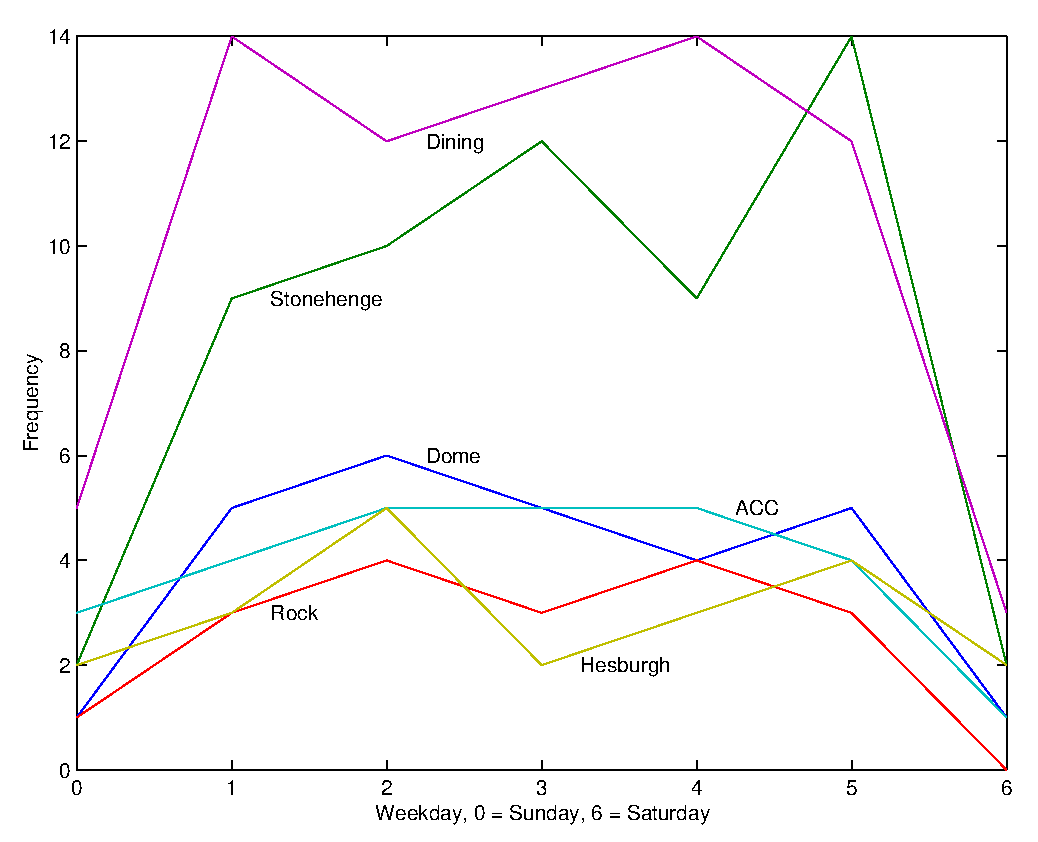
\includegraphics[scale=0.8]{sample_nd}}
%    \caption{Location distributions by day of where, where the X axis
%      is the weekday (0 through 6), and the Y axis is the sighting
%      frequency}
%    \label{fig:bogus3}
%  \end{center}
%\end{figure}
%
%Gnus typically tend to come out when there are large gatherings of
%humans with food.  Gnus work very hard at providing us with all the
%things that we like (trees, dirt, air, etc.), and so we should freely
%give them food.  They will come up and stand a respectful distance
%away from you, waiting to see if they will be rewarded for their
%efforts.  If you offer some food, they will take it and back off a
%respectful distance in order to consume their food while leaving you
%to your ``personal space.''  

%\section{Groovin' Gnus}
%\label{sec:groovin-gnus}
%
%Gnus do tend to stay away from humans in their normal day-to-day
%workings.  This is mainly because humans don't, for the most part,
%understand what they are doing.  If a Gnu is working, and a human
%approaches it, the Gnu will tend to drop whatever it is doing and run
%away.  This is probably do to the tendency for humans to have ``group
%meetings'' and ``productivity seminars.''  Most Gnus are deathly
%afraid of such overmanagement, and run at the slightest hint of it,
%for fear that it will cripple their real work.
%
%It is interesting, however, that Gnus have chosen an Institution of
%Higher Education for their BOO.\footnote{Base of Operations.}  It is
%often said that:
%\begin{quote}
%  Academic politics are the dirtiest, meanest, ugliest, and generally
%  the most low-down, in-your-face, and kick-em-while-they're-down than
%  anywhere else (even Washington D.C.)  because the stakes are so low.
%\end{quote}
%It has been hypothesized that the Gnus are subtly trying to affect a
%change for the better (i.e., eliminating the overmanagement problems)
%by working the very system that they are trying to change, from
%within.  That is, the graduates from Notre Dame can learn from the
%examples of the Gnus here, and run screaming (or chattering) at the
%slightest hint of overmanagement, and let the real work proceed
%unhindered.

% % uncomment the following lines,
% if using chapter-wise bibliography
%
% \bibliographystyle{ndnatbib}
% \bibliography{example}